% Options for packages loaded elsewhere
\PassOptionsToPackage{unicode}{hyperref}
\PassOptionsToPackage{hyphens}{url}
\PassOptionsToPackage{dvipsnames,svgnames,x11names}{xcolor}
%
\documentclass[
  letterpaper,
  DIV=11,
  numbers=noendperiod]{scrreprt}

\usepackage{amsmath,amssymb}
\usepackage{iftex}
\ifPDFTeX
  \usepackage[T1]{fontenc}
  \usepackage[utf8]{inputenc}
  \usepackage{textcomp} % provide euro and other symbols
\else % if luatex or xetex
  \usepackage{unicode-math}
  \defaultfontfeatures{Scale=MatchLowercase}
  \defaultfontfeatures[\rmfamily]{Ligatures=TeX,Scale=1}
\fi
\usepackage{lmodern}
\ifPDFTeX\else  
    % xetex/luatex font selection
\fi
% Use upquote if available, for straight quotes in verbatim environments
\IfFileExists{upquote.sty}{\usepackage{upquote}}{}
\IfFileExists{microtype.sty}{% use microtype if available
  \usepackage[]{microtype}
  \UseMicrotypeSet[protrusion]{basicmath} % disable protrusion for tt fonts
}{}
\makeatletter
\@ifundefined{KOMAClassName}{% if non-KOMA class
  \IfFileExists{parskip.sty}{%
    \usepackage{parskip}
  }{% else
    \setlength{\parindent}{0pt}
    \setlength{\parskip}{6pt plus 2pt minus 1pt}}
}{% if KOMA class
  \KOMAoptions{parskip=half}}
\makeatother
\usepackage{xcolor}
\setlength{\emergencystretch}{3em} % prevent overfull lines
\setcounter{secnumdepth}{5}
% Make \paragraph and \subparagraph free-standing
\ifx\paragraph\undefined\else
  \let\oldparagraph\paragraph
  \renewcommand{\paragraph}[1]{\oldparagraph{#1}\mbox{}}
\fi
\ifx\subparagraph\undefined\else
  \let\oldsubparagraph\subparagraph
  \renewcommand{\subparagraph}[1]{\oldsubparagraph{#1}\mbox{}}
\fi

\usepackage{color}
\usepackage{fancyvrb}
\newcommand{\VerbBar}{|}
\newcommand{\VERB}{\Verb[commandchars=\\\{\}]}
\DefineVerbatimEnvironment{Highlighting}{Verbatim}{commandchars=\\\{\}}
% Add ',fontsize=\small' for more characters per line
\usepackage{framed}
\definecolor{shadecolor}{RGB}{241,243,245}
\newenvironment{Shaded}{\begin{snugshade}}{\end{snugshade}}
\newcommand{\AlertTok}[1]{\textcolor[rgb]{0.68,0.00,0.00}{#1}}
\newcommand{\AnnotationTok}[1]{\textcolor[rgb]{0.37,0.37,0.37}{#1}}
\newcommand{\AttributeTok}[1]{\textcolor[rgb]{0.40,0.45,0.13}{#1}}
\newcommand{\BaseNTok}[1]{\textcolor[rgb]{0.68,0.00,0.00}{#1}}
\newcommand{\BuiltInTok}[1]{\textcolor[rgb]{0.00,0.23,0.31}{#1}}
\newcommand{\CharTok}[1]{\textcolor[rgb]{0.13,0.47,0.30}{#1}}
\newcommand{\CommentTok}[1]{\textcolor[rgb]{0.37,0.37,0.37}{#1}}
\newcommand{\CommentVarTok}[1]{\textcolor[rgb]{0.37,0.37,0.37}{\textit{#1}}}
\newcommand{\ConstantTok}[1]{\textcolor[rgb]{0.56,0.35,0.01}{#1}}
\newcommand{\ControlFlowTok}[1]{\textcolor[rgb]{0.00,0.23,0.31}{#1}}
\newcommand{\DataTypeTok}[1]{\textcolor[rgb]{0.68,0.00,0.00}{#1}}
\newcommand{\DecValTok}[1]{\textcolor[rgb]{0.68,0.00,0.00}{#1}}
\newcommand{\DocumentationTok}[1]{\textcolor[rgb]{0.37,0.37,0.37}{\textit{#1}}}
\newcommand{\ErrorTok}[1]{\textcolor[rgb]{0.68,0.00,0.00}{#1}}
\newcommand{\ExtensionTok}[1]{\textcolor[rgb]{0.00,0.23,0.31}{#1}}
\newcommand{\FloatTok}[1]{\textcolor[rgb]{0.68,0.00,0.00}{#1}}
\newcommand{\FunctionTok}[1]{\textcolor[rgb]{0.28,0.35,0.67}{#1}}
\newcommand{\ImportTok}[1]{\textcolor[rgb]{0.00,0.46,0.62}{#1}}
\newcommand{\InformationTok}[1]{\textcolor[rgb]{0.37,0.37,0.37}{#1}}
\newcommand{\KeywordTok}[1]{\textcolor[rgb]{0.00,0.23,0.31}{#1}}
\newcommand{\NormalTok}[1]{\textcolor[rgb]{0.00,0.23,0.31}{#1}}
\newcommand{\OperatorTok}[1]{\textcolor[rgb]{0.37,0.37,0.37}{#1}}
\newcommand{\OtherTok}[1]{\textcolor[rgb]{0.00,0.23,0.31}{#1}}
\newcommand{\PreprocessorTok}[1]{\textcolor[rgb]{0.68,0.00,0.00}{#1}}
\newcommand{\RegionMarkerTok}[1]{\textcolor[rgb]{0.00,0.23,0.31}{#1}}
\newcommand{\SpecialCharTok}[1]{\textcolor[rgb]{0.37,0.37,0.37}{#1}}
\newcommand{\SpecialStringTok}[1]{\textcolor[rgb]{0.13,0.47,0.30}{#1}}
\newcommand{\StringTok}[1]{\textcolor[rgb]{0.13,0.47,0.30}{#1}}
\newcommand{\VariableTok}[1]{\textcolor[rgb]{0.07,0.07,0.07}{#1}}
\newcommand{\VerbatimStringTok}[1]{\textcolor[rgb]{0.13,0.47,0.30}{#1}}
\newcommand{\WarningTok}[1]{\textcolor[rgb]{0.37,0.37,0.37}{\textit{#1}}}

\providecommand{\tightlist}{%
  \setlength{\itemsep}{0pt}\setlength{\parskip}{0pt}}\usepackage{longtable,booktabs,array}
\usepackage{calc} % for calculating minipage widths
% Correct order of tables after \paragraph or \subparagraph
\usepackage{etoolbox}
\makeatletter
\patchcmd\longtable{\par}{\if@noskipsec\mbox{}\fi\par}{}{}
\makeatother
% Allow footnotes in longtable head/foot
\IfFileExists{footnotehyper.sty}{\usepackage{footnotehyper}}{\usepackage{footnote}}
\makesavenoteenv{longtable}
\usepackage{graphicx}
\makeatletter
\def\maxwidth{\ifdim\Gin@nat@width>\linewidth\linewidth\else\Gin@nat@width\fi}
\def\maxheight{\ifdim\Gin@nat@height>\textheight\textheight\else\Gin@nat@height\fi}
\makeatother
% Scale images if necessary, so that they will not overflow the page
% margins by default, and it is still possible to overwrite the defaults
% using explicit options in \includegraphics[width, height, ...]{}
\setkeys{Gin}{width=\maxwidth,height=\maxheight,keepaspectratio}
% Set default figure placement to htbp
\makeatletter
\def\fps@figure{htbp}
\makeatother
\newlength{\cslhangindent}
\setlength{\cslhangindent}{1.5em}
\newlength{\csllabelwidth}
\setlength{\csllabelwidth}{3em}
\newlength{\cslentryspacingunit} % times entry-spacing
\setlength{\cslentryspacingunit}{\parskip}
\newenvironment{CSLReferences}[2] % #1 hanging-ident, #2 entry spacing
 {% don't indent paragraphs
  \setlength{\parindent}{0pt}
  % turn on hanging indent if param 1 is 1
  \ifodd #1
  \let\oldpar\par
  \def\par{\hangindent=\cslhangindent\oldpar}
  \fi
  % set entry spacing
  \setlength{\parskip}{#2\cslentryspacingunit}
 }%
 {}
\usepackage{calc}
\newcommand{\CSLBlock}[1]{#1\hfill\break}
\newcommand{\CSLLeftMargin}[1]{\parbox[t]{\csllabelwidth}{#1}}
\newcommand{\CSLRightInline}[1]{\parbox[t]{\linewidth - \csllabelwidth}{#1}\break}
\newcommand{\CSLIndent}[1]{\hspace{\cslhangindent}#1}

\usepackage{booktabs}
\usepackage{caption}
\usepackage{longtable}
\KOMAoption{captions}{tableheading}
\makeatletter
\makeatother
\makeatletter
\@ifpackageloaded{bookmark}{}{\usepackage{bookmark}}
\makeatother
\makeatletter
\@ifpackageloaded{caption}{}{\usepackage{caption}}
\AtBeginDocument{%
\ifdefined\contentsname
  \renewcommand*\contentsname{Table of contents}
\else
  \newcommand\contentsname{Table of contents}
\fi
\ifdefined\listfigurename
  \renewcommand*\listfigurename{List of Figures}
\else
  \newcommand\listfigurename{List of Figures}
\fi
\ifdefined\listtablename
  \renewcommand*\listtablename{List of Tables}
\else
  \newcommand\listtablename{List of Tables}
\fi
\ifdefined\figurename
  \renewcommand*\figurename{Figure}
\else
  \newcommand\figurename{Figure}
\fi
\ifdefined\tablename
  \renewcommand*\tablename{Table}
\else
  \newcommand\tablename{Table}
\fi
}
\@ifpackageloaded{float}{}{\usepackage{float}}
\floatstyle{ruled}
\@ifundefined{c@chapter}{\newfloat{codelisting}{h}{lop}}{\newfloat{codelisting}{h}{lop}[chapter]}
\floatname{codelisting}{Listing}
\newcommand*\listoflistings{\listof{codelisting}{List of Listings}}
\makeatother
\makeatletter
\@ifpackageloaded{caption}{}{\usepackage{caption}}
\@ifpackageloaded{subcaption}{}{\usepackage{subcaption}}
\makeatother
\makeatletter
\@ifpackageloaded{tcolorbox}{}{\usepackage[skins,breakable]{tcolorbox}}
\makeatother
\makeatletter
\@ifundefined{shadecolor}{\definecolor{shadecolor}{rgb}{.97, .97, .97}}
\makeatother
\makeatletter
\makeatother
\makeatletter
\makeatother
\ifLuaTeX
  \usepackage{selnolig}  % disable illegal ligatures
\fi
\IfFileExists{bookmark.sty}{\usepackage{bookmark}}{\usepackage{hyperref}}
\IfFileExists{xurl.sty}{\usepackage{xurl}}{} % add URL line breaks if available
\urlstyle{same} % disable monospaced font for URLs
\hypersetup{
  pdftitle={HIVCAre Documentation},
  pdfauthor={Bastian Reiter},
  colorlinks=true,
  linkcolor={blue},
  filecolor={Maroon},
  citecolor={Blue},
  urlcolor={Blue},
  pdfcreator={LaTeX via pandoc}}

\title{HIVCAre Documentation}
\usepackage{etoolbox}
\makeatletter
\providecommand{\subtitle}[1]{% add subtitle to \maketitle
  \apptocmd{\@title}{\par {\large #1 \par}}{}{}
}
\makeatother
\subtitle{Epidemiology and Inpatient Care Characteristics of
HIV-positive Cancer Patients in German university hospitals}
\author{Bastian Reiter}
\date{2023-08-03}

\begin{document}
\maketitle
\ifdefined\Shaded\renewenvironment{Shaded}{\begin{tcolorbox}[borderline west={3pt}{0pt}{shadecolor}, interior hidden, enhanced, boxrule=0pt, sharp corners, breakable, frame hidden]}{\end{tcolorbox}}\fi

\renewcommand*\contentsname{Table of contents}
{
\hypersetup{linkcolor=}
\setcounter{tocdepth}{2}
\tableofcontents
}
\bookmarksetup{startatroot}

\hypertarget{about-this-documentation}{%
\chapter{About This Documentation}\label{about-this-documentation}}

\hfill\break

This Research Documentation means to provide both a comprehensive source
of information about the underlying project as well as facilitate its
cooperative approach. Following the general ideas of
\href{https://www.fosteropenscience.eu/learning/what-is-open-science/\#/id/5ab8ea32dd1827131b90e3ac}{Open
Science}, we thus hope to achieve a high degree of transparency and
reproducibility in our conduct of research.

The design of this Documentation follows the guides on
\href{https://www.dgepi.de/assets/Good-Epidemiological-Practice-GEP-EurJ-Epidemiol-2019.pdf}{Good
Epidemiological Practice (GEP)}\textsuperscript{1} and
\href{https://www.dgepi.de/assets/Leitlinien-und-Empfehlungen/GPS_revision2-final_august2014.pdf}{Gute
Praxis Sekundärdatenanalyse (GPS)}\textsuperscript{2}.

\hfill\break

\hypertarget{guiding-principles}{%
\section{Guiding Principles}\label{guiding-principles}}

\href{https://www.fosteropenscience.eu/learning/what-is-open-science/\#/id/5ab8ea32dd1827131b90e3ac}{Open
Science Principles}

\href{https://www.dgepi.de/assets/Good-Epidemiological-Practice-GEP-EurJ-Epidemiol-2019.pdf}{Good
Epidemiological Practice (GPE)}

\href{https://www.dgepi.de/assets/Leitlinien-und-Empfehlungen/GPS_revision2-final_august2014.pdf}{Gute
Praxis Sekundärdatenanalyse (GPS)}

\href{https://www.go-fair.org/fair-principles/}{FAIR
Principles}\textsuperscript{3}

\href{https://www.strobe-statement.org/}{STROBE Statement}

\part{Project Information}

\hypertarget{project-synopsis}{%
\chapter{Project Synopsis}\label{project-synopsis}}

\hypertarget{section-ProjectBackground}{%
\section{Project Background}\label{section-ProjectBackground}}

\begin{itemize}
\item
  Infection with Human Immunodeficiency Virus (HIV) and its
  consequential acquired immune deficiency syndrome (AIDS) entail an
  increased risk of developing cancer. The associated malignancies are
  commonly classified into AIDS-defining cancer (AD, e.g.~Kaposi
  sarcoma) and HIV-associated non-AIDS-defining cancer (NAD,
  e.g.~Hodgkin lymphoma).
\item
  Establishment of effective antiretroviral therapy (ART) is considered
  a major driver of the steep decline in AD cancer incidence since the
  1990s, however the risk of NAD cancer in persons living with HIV
  (PLWH) remains elevated compared to non-infected individuals. Today
  cancer is the leading cause of death among the infected population, a
  fact that has in part been attributed to the considerable rise in life
  expectancy.
\item
  Medical care of HIV-positive cancer patients involves management of
  complex interactions between ART and potential side effects,
  anti-infective therapy as well as cancer treatment in a latently
  immunocompromised host.
\item
  Currently no specific care structures have been established in German
  hospitals to meet this medical challenge.
\item
  Exploration of Real World Data could provide insights into
  epidemiology and inpatient care characteristics of HIV-positive cancer
  patients.
\item
  We analyze data curated in the context of a federal law
  (Krankenhausentgeltgesetz, KHEntgG), that requires all German
  hospitals to transmit the so-called §21-data-set to a semi-public
  institute (InEK GmbH) under management of central health system
  organization.
\item
  The correspondent data base is curated and hosted by hospital
  infrastructure and can be accessed by Data Integration Centers.
\item
  Using federated analysis techniques ensures a high level of data
  privacy and maintains data sovereignty of the participating sites.
\end{itemize}

\hypertarget{project-governance}{%
\chapter{Project Governance}\label{project-governance}}

\hfill\break

\hypertarget{full-project-title}{%
\section{Full Project Title}\label{full-project-title}}

\textbf{Epidemiology and Inpatient Care Characteristics of HIV-positive
Cancer Patients in German university hospitals: A Real World Data
Exploration (HIVCAre).}

\hypertarget{project-initiation}{%
\section{Project Initiation}\label{project-initiation}}

\textbf{Prof.~Dr.~Jörg Janne Vehreschild\\
Melanie Stecher, PhD\\
Stefanie Andreas, M.Sc.\\
Dr.~Daniel Maier}

\hypertarget{project-supervision}{%
\section{Project Supervision}\label{project-supervision}}

\textbf{Prof.~Dr.~Jörg Janne Vehreschild}\\
{Department of Medicine\\
Hematology and Medical Oncology\\
University Hospital Frankfurt\\
Goethe University Frankfurt}

\hypertarget{project-administration}{%
\section{Project Administration}\label{project-administration}}

\textbf{Bastian Reiter}\\
{Department of Medicine\\
Hematology and Medical Oncology\\
University Hospital Frankfurt\\
Goethe University Frankfurt}

\hypertarget{research-associates}{%
\section{Research Associates}\label{research-associates}}

\begin{longtable*}{lllll}
\toprule
Last Name & First Name & Primary Affiliation & City & Author Contributions \\ 
\midrule
Albashiti & Fady & MeDIC LMU, Zentrum für Medizinische Datenintegration und -analyse, University Hospital Munich (LMU), Munich & Munich & Site data management \\ 
Andreas & Stefanie & Department of Medicine, Hematology and Medical Oncology, University Hospital Frankfurt, Goethe University, Frankfurt & Frankfurt & Project management, Site data management \\ 
Aubele & Fabio & MeDIC LMU, Zentrum für Medizinische Datenintegration und -analyse, University Hospital Munich (LMU), Munich & Munich & Site data management \\ 
Hagedorn & Marlien & MeDIC LMU, Zentrum für Medizinische Datenintegration und -analyse, University Hospital Munich (LMU), Munich & Munich & Site data management \\ 
Laukhuf & Andrea & Data Integration Center, University Hospital Freiburg, Freiburg & Freiburg & Site data management \\ 
Maier & Daniel & Department of Medicine, Hematology and Medical Oncology, University Hospital Frankfurt, Goethe University, Frankfurt & Frankfurt & Project management, Site data management \\ 
Müller & Matthias & Department of Internal Medicine 2, Infectious Diseases, University Hospital Freiburg, Freiburg & Freiburg & Site administration \\ 
Reiter & Bastian & Department of Medicine, Hematology and Medical Oncology, University Hospital Frankfurt, Goethe University, Frankfurt & Frankfurt & Project management, Data analysis \\ 
Roider & Julia & Division of Infectious Diseases, University Hospital Munich (LMU), Munich & Munich & Site administration \\ 
Sauer & Gabriel & Department of Internal Medicine I, University Hospital of Cologne, Cologne & Cologne & Site data management \\ 
Schulze & Nick & German Centre for Infection Research (DZIF), Partner Site Bonn-Cologne, Cologne & Cologne & Site data management \\ 
Seybold & Ulrich & Division of Infectious Diseases, University Hospital Munich (LMU), Munich & Munich & Site administration \\ 
Stecher & Melanie & Norwegian Institute of Public Health, Oslo & Oslo & Project initiation \\ 
Stephan & Christoph & HIVCENTER, Medical HIV Treatment and Research Unit, Johann Wolfgang Goethe University Frankfurt, Frankfurt & Frankfurt &  \\ 
Vehreschild & Jörg Janne & Department of Medicine, Hematology and Medical Oncology, University Hospital Frankfurt, Goethe University, Frankfurt & Frankfurt & Project initiation, Project supervision \\ 
Wehrle & Julius & Data Integration Center, University Hospital Freiburg, Freiburg & Freiburg & Site data management \\ 
\bottomrule
\end{longtable*}

\hypertarget{participating-institutions}{%
\section{Participating Institutions}\label{participating-institutions}}

\begin{longtable*}{llll}
\toprule
City & Hospital & University & Institution \\ 
\midrule
Cologne & Uniklinik Köln & Universität zu Köln & Medical Data Integration Center (MeDIC) \\ 
Frankfurt/Main & Universitätsklinikum Frankfurt & Goethe-Universität Frankfurt & Datenintegrationszentrum (DIZ) \\ 
Freiburg & Universitätsklinikum Freiburg & Albert-Ludwigs-Universität Freiburg & Datenintegrationszentrum (DIZ) \\ 
Munich & LMU Klinikum & Ludwig-Maximilians-Universität & Zentrum für Medizinische Datenintegration und -analyse (MeDICLMU) \\ 
\bottomrule
\end{longtable*}

\hypertarget{funding}{%
\section{Funding}\label{funding}}

There is no third-party funding for this project.

\hypertarget{conflicts-of-interest}{%
\section{Conflicts of Interest}\label{conflicts-of-interest}}

We have no conflicts of interest to disclose.

\hypertarget{publication}{%
\section{Publication}\label{publication}}

The study results will be published in cooperation with all associates.

\hypertarget{study-design}{%
\chapter{Study Design}\label{study-design}}

\begin{quote}
\textbf{HIVCAre} is a multicenter retrospective cohort study, conducted
on Real World Health Data from German university hospitals.
\end{quote}

\hypertarget{section-ResearchObjectives}{%
\section{Research Objectives}\label{section-ResearchObjectives}}

\begin{quote}
\textbf{Main Objective:} Explore epidemiology and inpatient care
characteristics of HIV-positive cancer patients
\end{quote}

\begin{itemize}
\item
  Describe cancer occurrence in HIV-positive patients over time
  stratified by cancer category
\item
  Explore possible differences in care characteristics between
  HIV-negative and HIV-positive cancer patients
\item
  Explore differences in course of therapy between HIV-negative and
  HIV-positive cancer patients
\end{itemize}

For a detailed list of Research Items, see according Section
\protect\hyperlink{section-ResearchItems}{below}.

\hypertarget{study-data}{%
\section{Study Data}\label{study-data}}

The primary health data analyzed in this study is curated by hospitals
following legal requirements founded in
\href{https://www.gesetze-im-internet.de/khentgg/__21.html}{§21
Krankenhausentgeltgesetz (KHEntgG)}. For more details, see Chapter
\protect\hyperlink{chapter-StudyData}{Study Data}.

\hypertarget{section-StudyCohort}{%
\section{Study Cohort}\label{section-StudyCohort}}

Data of patients admitted to the following university hospitals (in
alphabetical order):

\begin{longtable*}{lll}
\toprule
City & Hospital & University \\ 
\midrule
Cologne & Uniklinik Köln & Universität zu Köln \\ 
Frankfurt/Main & Universitätsklinikum Frankfurt & Goethe-Universität Frankfurt \\ 
Freiburg & Universitätsklinikum Freiburg & Albert-Ludwigs-Universität Freiburg \\ 
Munich & LMU Klinikum & Ludwig-Maximilians-Universität \\ 
\bottomrule
\end{longtable*}

\hypertarget{inclusion-criteria}{%
\subsubsection{Inclusion criteria}\label{inclusion-criteria}}

\begin{itemize}
\tightlist
\item
  Admitted between 01-01-2005 and 12-31-2019
\item
  Aged at least 18 years at date of admission
\item
  At least one documented ICD-10 code representing malignancy or HIV
  infection
\end{itemize}

\hypertarget{exclusion-criteria}{%
\subsubsection{Exclusion criteria}\label{exclusion-criteria}}

\begin{itemize}
\tightlist
\item
  Implausible documentation of ICD-10 codes
\end{itemize}

\hfill\break

\hypertarget{stratification-model}{%
\subsection{Stratification Model}\label{stratification-model}}

\begin{figure}

{\centering 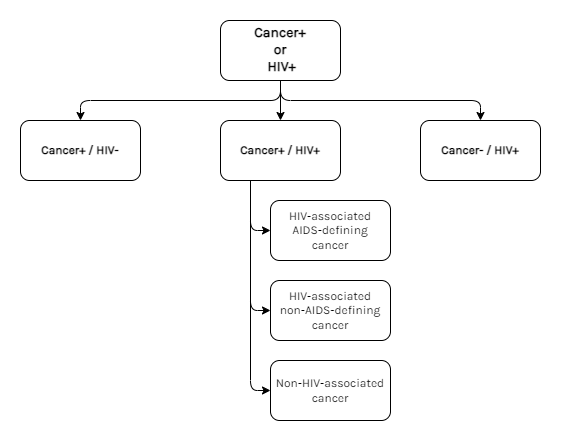
\includegraphics{Images/StratificationModel.png}

}

\end{figure}

\hypertarget{sample-size-determination}{%
\section{Sample Size Determination}\label{sample-size-determination}}

Since this study does not aim at a particular effect size analysis and
it can be assumed that the yielded Sample Sizes will be rather large, no
specific Sample Size Determination will be performed.

\hypertarget{section-ResearchItems}{%
\section{Research Items}\label{section-ResearchItems}}

The following research items result from the research objectives stated
\protect\hyperlink{section-ResearchObjectives}{here}.

\begin{longtable*}{rlllll}
\toprule
Item & Compared Strata & Research Item & Metrum Specification & Method Type & Method \\ 
\midrule
\multicolumn{6}{l}{Epidemiology} \\ 
\midrule
1 & All main subgroups & Sample size over time &  & Descriptive & Stacked Histogram \\ 
2 & All main subgroups & Age distribution over time & Age at first occurrence of primary diagnosis & Descriptive & Stacked Histogram \\ 
3 & All main subgroups & Gender distribution over time &  & Descriptive & Stacked Histogram \\ 
4 & All main subgroups & Spatial distribution & Counts of patients from different postal code areas & Descriptive & Map \\ 
7 & Cancer+/HIV+ & Occurrence of different HIV-associated cancer diagnoses over time &  & Descriptive & Stacked Histogram \\ 
8 & Cancer+/HIV- & Occurrence of different HIV-associated cancer diagnoses over time for control &  & Descriptive & Stacked Histogram (for control) \\ 
9 & Cancer+/HIV+ & Projection of HIV-associated cancer diagnoses &  & Inferential & Regression \\ 
10 & Cancer+/HIV+ & Occurrence of AIDS in cancer patients, stratified by cancer category over time &  & Descriptive & Stacked Histogram \\ 
11 & Cancer+/HIV+ & Occurrence of AIDS code after chemotherapy &  & Descriptive &  \\ 
12 & Cancer+/HIV+ & Presumed order of diagnosis of HIV infection and cancer over time &  & Descriptive & Stacked Histogram \\ 
13 & Cancer+/HIV- vs. Cancer+/HIV+ & Age at presumed cancer onset & Age at first cancer code occurrence & Descriptive &  \\ 
14 & Cancer+/HIV- vs. Cancer+/HIV+ & Cancer topography grouped by organ &  & Descriptive & Pyramid plot \\ 
15 & Cancer+/HIV- vs. Cancer+/HIV+ & Cancer topography grouped by organ over time &  & Descriptive & Stacked Histogram \\ 
16 & Cancer+/HIV- vs. Cancer+/HIV+ & Projection of cancer topography grouped by organ &  & Inferential & Regression \\ 
17 & Cancer+/HIV- vs. Cancer+/HIV+ & Cancer topography grouped by ICD-10 grouping &  & Descriptive & Pyramid plot \\ 
18 & Cancer+/HIV- vs. Cancer+/HIV+ & Cancer topography grouped by ICD-10 grouping over time &  & Descriptive & Stacked Histogram \\ 
19 & Cancer+/HIV- vs. Cancer+/HIV+ & Projection of cancer topography grouped by ICD-10 grouping &  & Inferential & Regression \\ 
20 & Cancer+/HIV- vs. Cancer+/HIV+ & Cancer occurrence grouped by entity &  & Descriptive & Table / Pyramid plot of most common \\ 
21 & Cancer+/HIV- vs. Cancer+/HIV+ & Cancer occurrence grouped by entity over time &  & Descriptive & Table / Stacked histogram of most common \\ 
22 & Cancer+/HIV- vs. Cancer+/HIV+ & Projection of cancer occurrence grouped by entity &  & Inferential & Regression \\ 
25 & Cancer+/HIV- vs. Cancer+/HIV+ & Metastasis occurrence &  & Descriptive & Columnplot \\ 
31 & Cancer+ & Sequence in presumed HIV / Cancer / Metastasis / AIDS onset &  & Descriptive & Sankey diagram \\ 
\midrule
\multicolumn{6}{l}{Care Characteristics} \\ 
\midrule
5 & All main subgroups & Count of admissions per patient &  & Descriptive & Boxplot \\ 
6 & All main subgroups & Mean length of stay per patient &  & Descriptive & Box-/Violinplot \\ 
\midrule
\multicolumn{6}{l}{Therapy} \\ 
\midrule
23 & Cancer+/HIV- vs. Cancer+/HIV+ & Occurrence of cancer therapy modalities &  & Descriptive & Columnplot \\ 
24 & Cancer+/HIV- vs. Cancer+/HIV+ & Count of chemotherapy sessions &  & Descriptive &  \\ 
27 & Cancer+/HIV- vs. Cancer+/HIV+ & Occurrence of complications after chemotherapy & Complications: Ventilation, dialysis & Descriptive &  \\ 
28 & Cancer+/HIV- vs. Cancer+/HIV+ & Time from chemotherapy to complication &  & Descriptive, Inferential & Kaplan-Meier-Plot for cumulative hazard \\ 
32 & Cancer+/HIV- & Sequence of cancer therapy modalities &  & Descriptive & Sankey diagram \\ 
33 & Cancer+/HIV+ & Sequence of cancer therapy modalities &  & Descriptive & Sankey diagram \\ 
\midrule
\multicolumn{6}{l}{Outcome} \\ 
\midrule
26 & Cancer+/HIV- vs. Cancer+/HIV+ & Time from presumed cancer to presumed metastasis onset &  & Desriptive, Inferential & Kaplan-Meier-Plot for cumulative hazard \\ 
29 & Cancer+/HIV- vs. Cancer+/HIV+ & Death after chemotherapy &  & Descriptive &  \\ 
30 & Cancer+/HIV- vs. Cancer+/HIV+ & Discharge reasons &  & Descriptive, Inferential &  \\ 
\bottomrule
\end{longtable*}

\hypertarget{study-data-1}{%
\chapter{Study Data}\label{study-data-1}}

\hfill\break

\hypertarget{data-generation}{%
\section{Data Generation}\label{data-generation}}

Primarily, data accumulated in the context of a federal law called
\emph{Krankenhausentgeltgesetz} (KHEntgG) is used to conduct this study.
The KHEntgG requires all German hospitals to transmit the so-called
§21-data-set to a semi-public institute (InEK GmbH) under management of
central health system organizations.\\
For more information, see
\href{https://www.g-drg.de/datenlieferung-gem.-21-khentgg/datenlieferung-gem.-21-abs.1-khentgg/dokumente-zur-datenlieferung/dokumente-zur-datenlieferung}{here}.

\hypertarget{data-storage-and-administration}{%
\section{Data Storage and
Administration}\label{data-storage-and-administration}}

The data to be analyzed in this project is stored and administered by
Data Integration Centers (DIC) of the participating university
hospitals. No individual-level patient data will be transmitted (see
Section on \protect\hyperlink{section-FederatedAnalysis}{Federated
Analysis}). For a detailed insight into the requested Study Data see
Chapter \protect\hyperlink{chapter-DataSelection}{Data Selection}.

\hypertarget{section-FederatedAnalysis}{%
\section{Federated Analysis}\label{section-FederatedAnalysis}}

This study applies methods of Federated Data Analysis, with the
following key consequences:

\begin{itemize}
\tightlist
\item
  Individual-level data is solely accessed by institutions of the
  participating sites.
\item
  An analytic procedure (usually in the form of an executable Analysis
  Script) is provided to the sites by the Project Manager.
\item
  The analytic output (usually in the form of aggregated data) is
  transmitted to the Project Manager
\end{itemize}

\hypertarget{data-privacy-and-security}{%
\section{Data Privacy and Security}\label{data-privacy-and-security}}

For individual-level data, the following applies: * It is pseudonymized
* No individual-level data accessed in this study will be transmitted
outside of the participating sites

For aggregated data, the following applies: * Various automated and
supervised measures are put in place to minimize risk of
re-identification * All files encrypted

\hypertarget{study-participant-consent}{%
\section{Study Participant Consent}\label{study-participant-consent}}

Since

\hypertarget{meta-data}{%
\section{Meta Data}\label{meta-data}}

\hypertarget{administration}{%
\chapter{Administration}\label{administration}}

\hypertarget{ethics-committee-votes}{%
\section{Ethics Committee Votes}\label{ethics-committee-votes}}

\hypertarget{use-and-access-request}{%
\section{Use and Access Request}\label{use-and-access-request}}

\hypertarget{roadmap}{%
\chapter{Roadmap}\label{roadmap}}

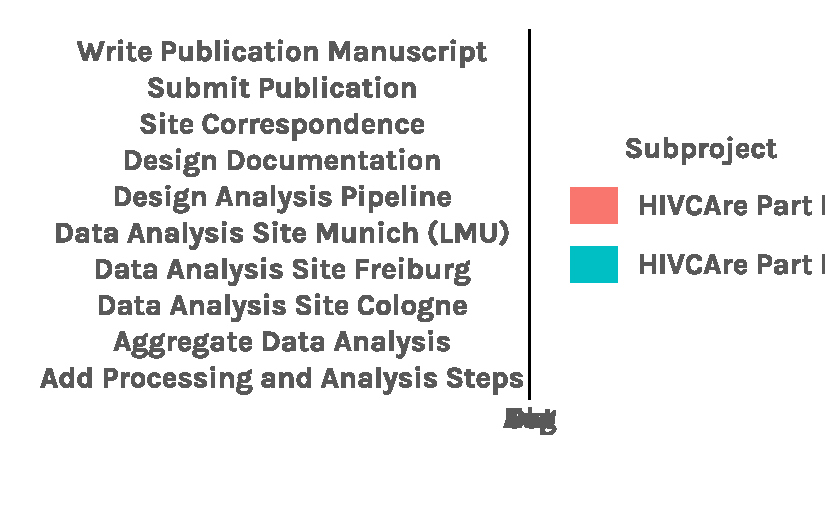
\includegraphics{Roadmap_files/figure-pdf/Roadmap-1.pdf}

\hypertarget{downloads}{%
\chapter{Downloads}\label{downloads}}

\hfill\break

\begin{longtable*}{cllc}
\toprule
File & Description & File Type & Source \\ 
\midrule
\multicolumn{4}{l}{Appended Documents} \\ 
\midrule
<a href="./Downloads/KHEntgG_UebermittlungVonDaten_2023.pdf" target="_blank">Anlage zur Vereinbarung über die Übermittlung von Daten nach §21 Abs. 4 und Abs. 5 KHEntgG</a> & Specification of data to be transmitted in the context of KHEntgG §21 (Version 2023) & PDF & <a href="https://www.g-drg.de/" target="_blank">Institut für das Entgeltsystem im Krankenhaus (InEK)</a> \\ 
<a href="./Downloads/ZI_HIVCodingManual_2023.pdf" target="_blank">Zi-Kodier-Manual HIV</a> & Established Manual for ICD-10 Coding of HIV Status and Diseases in Germany (Version 2023) & PDF & <a href="https://www.zi.de/" target="_blank">Zentralinstitut kassenärztliche Versorgung</a> \\ 
\midrule
\multicolumn{4}{l}{Meta Data} \\ 
\midrule
<a href="./Downloads/ICD10CancerGrouping.csv" target="_blank">Grouping of ICD-10 Cancer Codes</a> & Meta data on Grouping of cancer diagnoses according to ICD-10 & CSV & Bastian Reiter \\ 
<a href="./Downloads/ICD10HIVStatus.csv" target="_blank">ICD-10-Coding of HIV Status</a> & Meta data on valid ICD-10-Coding of HIV Status abiding by the ZI HIV Coding Manual & CSV & Bastian Reiter \\ 
<a href="./Downloads/ICD10HIVDiseases.csv" target="_blank">ICD-10-Coding of HIV-associated Diseases</a> & Meta data on valid ICD-10-Coding of HIV-associated Diseases abiding by the ZI HIV Coding Manual & CSV & Bastian Reiter \\ 
\bottomrule
\end{longtable*}

\part{Federated Analysis}

\hypertarget{general-cooperative-approach}{%
\chapter{General Cooperative
Approach}\label{general-cooperative-approach}}

\hfill\break

\hypertarget{proposed-process-of-cooperation}{%
\section{Proposed Process of
Cooperation}\label{proposed-process-of-cooperation}}

\begin{figure}

{\centering \includegraphics{Images/FedAnalysisApproach.png}

}

\end{figure}

\hypertarget{data-flow-in-analysis-pipeline-at-participating-sites}{%
\section{Data Flow in Analysis Pipeline at Participating
Sites}\label{data-flow-in-analysis-pipeline-at-participating-sites}}

\begin{figure}

{\centering \includegraphics[width=0.7\textwidth,height=\textheight]{Images/DataFlowSite.png}

}

\end{figure}

\hypertarget{data-flow-in-main-analysis-pipeline-at-site-of-project-administrator}{%
\section{Data Flow in Main Analysis Pipeline at Site of Project
Administrator}\label{data-flow-in-main-analysis-pipeline-at-site-of-project-administrator}}

\begin{figure}

{\centering \includegraphics[width=0.7\textwidth,height=\textheight]{Images/DataFlowMain.png}

}

\end{figure}

\hypertarget{data-selection}{%
\chapter{Data Selection}\label{data-selection}}

\hfill\break

\hypertarget{data-source-and-form}{%
\section{Data Source and Form}\label{data-source-and-form}}

The primary data source is a hospital's data base on KHEntgG-§21-data.
This data is usually accessible by the hospital's Data Integration
Center (DIC). Selected data should be exported to a tabular file format
like .csv oder .xlsx in order to be fed into the analysis pipeline
provided by the Project Administrator.

\hypertarget{cohort-selection}{%
\section{Cohort Selection}\label{cohort-selection}}

In accordance with the \protect\hyperlink{section-StudyCohort}{Study
Cohort specification} data of the following cases and their
corresponding patients should be selected from a local data base:

\begin{itemize}
\tightlist
\item
  Date of admission between 01-01-2005 and 12-31-2019
\item
  Age at date of admission at least 18 years
\item
  Select all cases of patients with one of the following ICD-10 codes
  documented in their case data:
\end{itemize}

\begin{longtable*}{ll}
\toprule
ICD-10 Code & Interpretation \\ 
\midrule
\multicolumn{2}{l}{Cancer} \\ 
\midrule
Starting with C & All malignant neoplasms (primary and secondary) \\ 
Starting with D0 & In-situ neoplasms \\ 
D37 - D48 & Neoplasms of uncertain / unknown behaviour \\ 
Z08 & Follow-up examination after treatment for malignant neoplasms \\ 
Z85, Z92.6 & Personal history of cancer / cancer therapy \\ 
\midrule
\multicolumn{2}{l}{HIV} \\ 
\midrule
B20 & Human immunodeficiency virus [HIV] disease resulting in infectious and parasitic diseases \\ 
B21 & Human immunodeficiency virus [HIV] disease resulting in malignant neoplasms \\ 
B22 & Human immunodeficiency virus [HIV] disease resulting in other specified diseases \\ 
B23.x & Human immunodeficiency virus [HIV] disease resulting in other conditions \\ 
B24 & Unspecified human immunodeficiency virus [HIV] disease \\ 
Z21 & Asymptomatic human immunodeficiency virus [HIV] infection status \\ 
O98.7 & Human immunodeficiency virus [HIV] disease complicating pregnancy, childbirth and the puerperium \\ 
U60.x & Clinical category of HIV disease \\ 
U61.x & Count of CD4+-T-cells per microliter blood \\ 
U85 & Human immunodeficiency virus with resistance against virostatics \\ 
\bottomrule
\end{longtable*}

\hypertarget{required-data-elements}{%
\section{Required Data Elements}\label{required-data-elements}}

The\ldots{}

Following the syntax and terminology used in the official addendum on
data transmission in compliance with §21 KHEntgG (see
\protect\hyperlink{chapter-Downloads}{Downloads}),

\begin{longtable*}{llll}
\toprule
Attribute Name & Attribute Description & Obligatory & Attribute Data Type \\ 
\midrule
\multicolumn{4}{l}{Table: Fall} \\ 
\midrule
KH-internes-Kennzeichen & Hospital-specific Case ID & yes & character \\ 
Geburtsjahr & Year of birth & yes & numeric \\ 
Geschlecht & Sex & yes & character \\ 
PLZ & Postal code & yes & character \\ 
Aufnahmedatum & Admission date & yes & date \\ 
Aufnahmeanlass & Admission cause & yes & character \\ 
Entlassungsdatum & Discharge date & yes & date \\ 
Entlassungsgrund & Discharge reason & yes & character \\ 
Alter-in-Jahren-am-Aufnahmetag & Age at admission date & no & numeric \\ 
Patientennummer & Hospital-specific Patient ID & yes & character \\ 
Verweildauer-Intensiv & Time spent in Intensive Care & yes & numeric \\ 
\midrule
\multicolumn{4}{l}{Table: FAB} \\ 
\midrule
Fachabteilung & Specialty department & yes & character \\ 
FAB-Aufnahmedatum & Admission date at Specialty department & yes & date \\ 
FAB-Entlassungsdatum & Discharge date at Specialty department & yes & date \\ 
KennungIntensivbett & Whether stay at Specialty department was in Intensive Care & yes & character \\ 
\midrule
\multicolumn{4}{l}{Table: ICD} \\ 
\midrule
Diagnoseart & Diagnosis type & yes & character \\ 
ICD-Version & ICD-10-GM Version & yes & numeric \\ 
ICD-Kode & ICD-10 Code & yes & character \\ 
Sekundär-Kode & Secondary ICD-10 Code & no & character \\ 
\midrule
\multicolumn{4}{l}{Table: OPS} \\ 
\midrule
OPS-Version & OPS Version & yes & numeric \\ 
OPS-Kode & OPS Code & yes & character \\ 
OPS-Datum & OPS Date & yes & date \\ 
\bottomrule
\end{longtable*}

\hypertarget{mockup-sql-query}{%
\section{Mockup SQL Query}\label{mockup-sql-query}}

A corresponding sequence of mockup SQL queries could look like the
following:

\begin{Shaded}
\begin{Highlighting}[]

\CommentTok{{-}{-} Create table *EligibleCases*: All Cases of eligible Patients (Subset of Table *Fall*) {-}{-}}
\KeywordTok{CREATE} \KeywordTok{TABLE}\NormalTok{ EligibleCases }\KeywordTok{AS}
\KeywordTok{SELECT}\NormalTok{ KH}\OperatorTok{{-}}\NormalTok{internes}\OperatorTok{{-}}\NormalTok{Kennzeichen,}
\NormalTok{       Geburtsjahr,}
\NormalTok{       Geschlecht,}
\NormalTok{       PLZ,}
\NormalTok{       Aufnahmedatum,}
\NormalTok{       Aufnahmeanlass,}
\NormalTok{       Entlassungsdatum,}
\NormalTok{       Entlassungsgrund,}
       \KeywordTok{Alter}\OperatorTok{{-}}\KeywordTok{in}\OperatorTok{{-}}\NormalTok{Jahren}\OperatorTok{{-}}\NormalTok{am}\OperatorTok{{-}}\NormalTok{Aufnahmetag,}
\NormalTok{       Patientennummer,}
\NormalTok{       Verweildauer}\OperatorTok{{-}}\NormalTok{Intensiv}
\KeywordTok{FROM}\NormalTok{ Fall}
\KeywordTok{WHERE}\NormalTok{ Patientennummer }\KeywordTok{IN}
\NormalTok{  ( }\KeywordTok{SELECT} \KeywordTok{DISTINCT}\NormalTok{ Patientennummer}
      \KeywordTok{FROM}\NormalTok{ Fall }\KeywordTok{LEFT} \KeywordTok{JOIN}\NormalTok{ ICD }\KeywordTok{ON}\NormalTok{ Fall.KH}\OperatorTok{{-}}\NormalTok{internes}\OperatorTok{{-}}\NormalTok{Kennzeichen }\OperatorTok{=}\NormalTok{ ICD.KH}\OperatorTok{{-}}\NormalTok{internes}\OperatorTok{{-}}\NormalTok{Kennzeichen}
      \KeywordTok{WHERE}\NormalTok{ Diagnoseschlüssel }\KeywordTok{LIKE} \StringTok{\textquotesingle{}C\%\textquotesingle{}}
         \KeywordTok{OR}\NormalTok{ Diagnoseschlüssel }\KeywordTok{LIKE} \StringTok{\textquotesingle{}D0\%\textquotesingle{}}
         \KeywordTok{OR}\NormalTok{ Diagnoseschlüssel }\KeywordTok{LIKE} \StringTok{\textquotesingle{}D3[7{-}9]\textquotesingle{}}
         \KeywordTok{OR}\NormalTok{ Diagnoseschlüssel }\KeywordTok{LIKE} \StringTok{\textquotesingle{}D4[0{-}8]\textquotesingle{}}
         \KeywordTok{OR}\NormalTok{ Diagnoseschlüssel }\KeywordTok{IN}\NormalTok{ (}\StringTok{\textquotesingle{}Z08\textquotesingle{}}\NormalTok{, }\StringTok{\textquotesingle{}Z85\textquotesingle{}}\NormalTok{, }\StringTok{\textquotesingle{}Z92.6\textquotesingle{}}\NormalTok{)}
         \KeywordTok{OR}\NormalTok{ Diagnoseschlüssel }\KeywordTok{IN}\NormalTok{ (}\StringTok{\textquotesingle{}B20\textquotesingle{}}\NormalTok{, }\StringTok{\textquotesingle{}B21\textquotesingle{}}\NormalTok{, }\StringTok{\textquotesingle{}B22\textquotesingle{}}\NormalTok{, }\StringTok{\textquotesingle{}B23.{-}\textquotesingle{}}\NormalTok{, }\StringTok{\textquotesingle{}B23.0\textquotesingle{}}\NormalTok{, }\StringTok{\textquotesingle{}B23.8\textquotesingle{}}\NormalTok{, }\StringTok{\textquotesingle{}B24\textquotesingle{}}\NormalTok{, }\StringTok{\textquotesingle{}Z21\textquotesingle{}}\NormalTok{, }\StringTok{\textquotesingle{}O98.7\textquotesingle{}}\NormalTok{)}
         \KeywordTok{OR}\NormalTok{ Sekundär}\OperatorTok{{-}}\NormalTok{Diagnoseschlüssel }\KeywordTok{LIKE} \StringTok{\textquotesingle{}U60\%\textquotesingle{}}
         \KeywordTok{OR}\NormalTok{ Sekundär}\OperatorTok{{-}}\NormalTok{Diagnoseschlüssel }\KeywordTok{LIKE} \StringTok{\textquotesingle{}U61\%\textquotesingle{}}
         \KeywordTok{OR}\NormalTok{ Sekundär}\OperatorTok{{-}}\NormalTok{Diagnoseschlüssel }\KeywordTok{LIKE} \StringTok{\textquotesingle{}U85\%\textquotesingle{}}\NormalTok{ )}


\CommentTok{{-}{-} Select subset of Table *FAB* for Export {-}{-}}
\KeywordTok{SELECT}\NormalTok{ FAB.KH}\OperatorTok{{-}}\NormalTok{internes}\OperatorTok{{-}}\NormalTok{Kennzeichen,}
\NormalTok{       FAB.Fachabteilung,}
\NormalTok{       FAB.FAB}\OperatorTok{{-}}\NormalTok{Aufnahmedatum,}
\NormalTok{       FAB.FAB}\OperatorTok{{-}}\NormalTok{Entlassungsdatum,}
\NormalTok{       FAB.KennungIntensivbett}
\KeywordTok{FROM}\NormalTok{ FAB }\KeywordTok{RIGHT} \KeywordTok{JOIN}\NormalTok{ EligibleCaseIDs }\KeywordTok{AS}
\NormalTok{                    ( }\KeywordTok{SELECT} \KeywordTok{DISTINCT}\NormalTok{ KH}\OperatorTok{{-}}\NormalTok{internes}\OperatorTok{{-}}\NormalTok{Kennzeichen }\KeywordTok{FROM}\NormalTok{ EligibleCases )}
         \KeywordTok{ON}\NormalTok{ FAB.KH}\OperatorTok{{-}}\NormalTok{internes}\OperatorTok{{-}}\NormalTok{Kennzeichen }\OperatorTok{=}\NormalTok{ EligibleCaseIDs.KH}\OperatorTok{{-}}\NormalTok{internes}\OperatorTok{{-}}\NormalTok{Kennzeichen}


\CommentTok{{-}{-} Select subset of Table *ICD* for Export {-}{-}}
\KeywordTok{SELECT}\NormalTok{ ICD.KH}\OperatorTok{{-}}\NormalTok{internes}\OperatorTok{{-}}\NormalTok{Kennzeichen,}
\NormalTok{       ICD.Diagnoseart,}
\NormalTok{       ICD.ICD}\OperatorTok{{-}}\NormalTok{Version,}
\NormalTok{       ICD.ICD}\OperatorTok{{-}}\NormalTok{Kode,}
\NormalTok{       ICD.Sekundär}\OperatorTok{{-}}\NormalTok{Kode}
\KeywordTok{FROM}\NormalTok{ ICD }\KeywordTok{RIGHT} \KeywordTok{JOIN}\NormalTok{ EligibleCaseIDs }\KeywordTok{AS}
\NormalTok{                    ( }\KeywordTok{SELECT} \KeywordTok{DISTINCT}\NormalTok{ KH}\OperatorTok{{-}}\NormalTok{internes}\OperatorTok{{-}}\NormalTok{Kennzeichen }\KeywordTok{FROM}\NormalTok{ EligibleCases )}
         \KeywordTok{ON}\NormalTok{ ICD.KH}\OperatorTok{{-}}\NormalTok{internes}\OperatorTok{{-}}\NormalTok{Kennzeichen }\OperatorTok{=}\NormalTok{ EligibleCaseIDs.KH}\OperatorTok{{-}}\NormalTok{internes}\OperatorTok{{-}}\NormalTok{Kennzeichen}


\CommentTok{{-}{-} Select subset of Table *OPS* for Export {-}{-}}
\KeywordTok{SELECT}\NormalTok{ OPS.KH}\OperatorTok{{-}}\NormalTok{internes}\OperatorTok{{-}}\NormalTok{Kennzeichen,}
\NormalTok{       OPS.OPS}\OperatorTok{{-}}\NormalTok{Version,}
\NormalTok{       OPS.OPS}\OperatorTok{{-}}\NormalTok{Kode,}
\NormalTok{       OPS.OPS}\OperatorTok{{-}}\NormalTok{Datum}
\KeywordTok{FROM}\NormalTok{ OPS }\KeywordTok{RIGHT} \KeywordTok{JOIN}\NormalTok{ EligibleCaseIDs }\KeywordTok{AS}
\NormalTok{                    ( }\KeywordTok{SELECT} \KeywordTok{DISTINCT}\NormalTok{ KH}\OperatorTok{{-}}\NormalTok{internes}\OperatorTok{{-}}\NormalTok{Kennzeichen }\KeywordTok{FROM}\NormalTok{ EligibleCases )}
         \KeywordTok{ON}\NormalTok{ OPS.KH}\OperatorTok{{-}}\NormalTok{internes}\OperatorTok{{-}}\NormalTok{Kennzeichen }\OperatorTok{=}\NormalTok{ EligibleCaseIDs.KH}\OperatorTok{{-}}\NormalTok{internes}\OperatorTok{{-}}\NormalTok{Kennzeichen}

\end{Highlighting}
\end{Shaded}

\hypertarget{script-execution}{%
\chapter{Script Execution}\label{script-execution}}

\hfill\break

\hypertarget{proceeding-of-analysis-execution}{%
\section{Proceeding of Analysis
Execution}\label{proceeding-of-analysis-execution}}

\begin{figure}

{\centering \includegraphics[width=0.7\textwidth,height=\textheight]{Images/FedAnalysisManual.png}

}

\end{figure}

\hypertarget{gitlab-repository}{%
\section{GitLab Repository}\label{gitlab-repository}}

\begin{figure}

{\centering 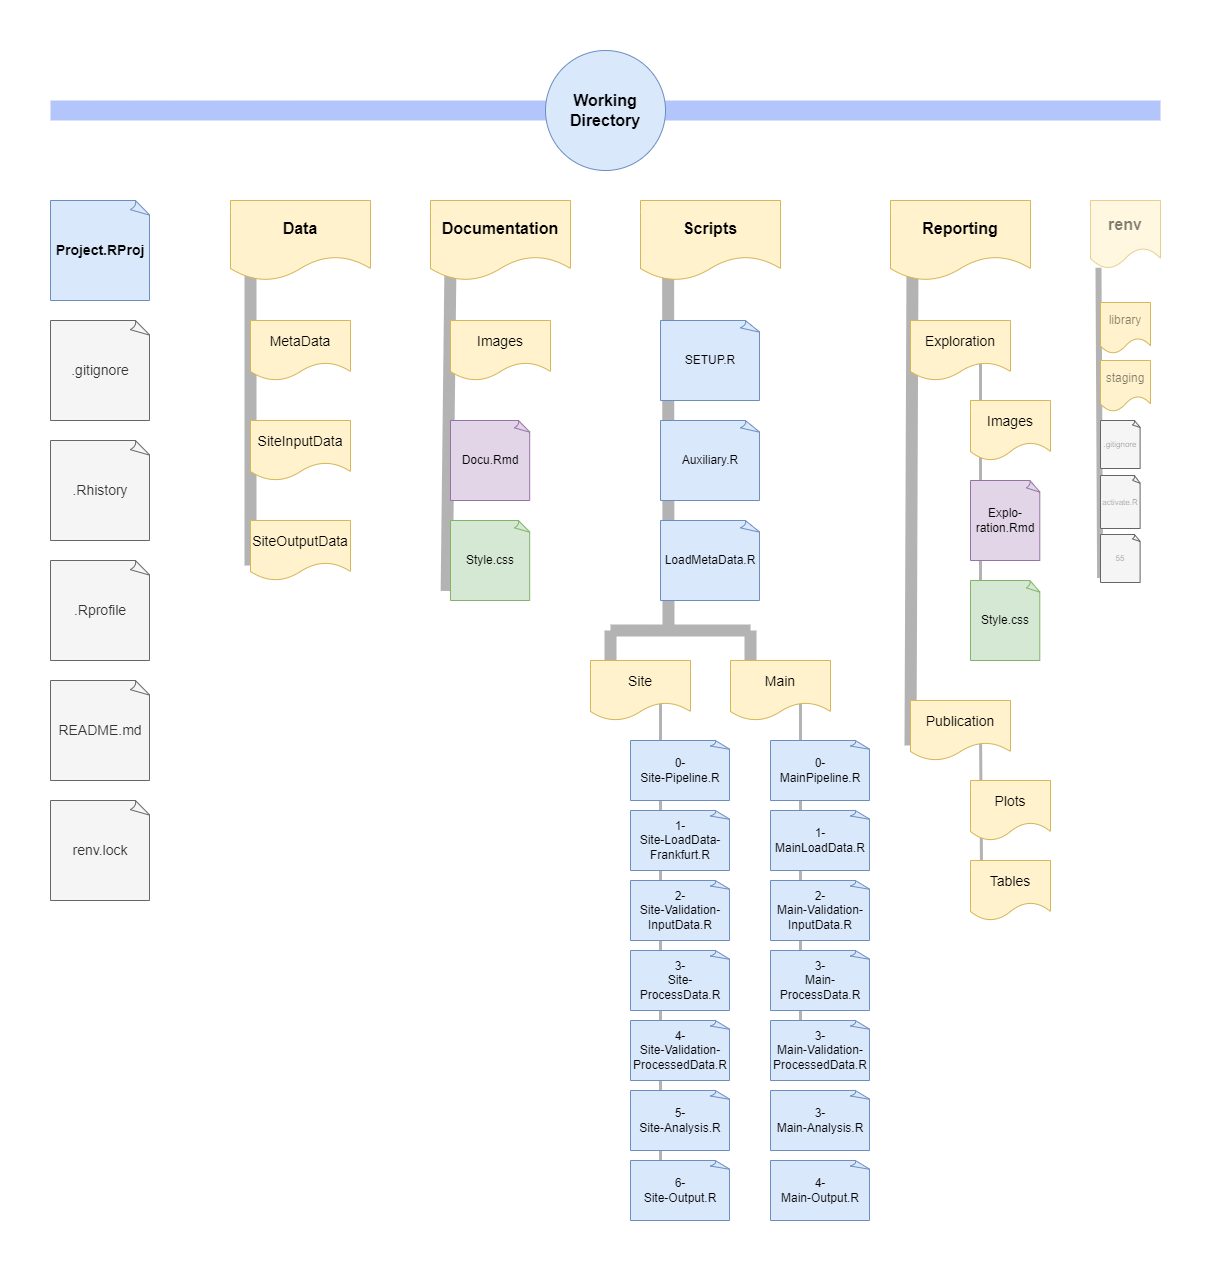
\includegraphics{Images/GitLabRepository.png}

}

\end{figure}

\hypertarget{runtime-environment}{%
\chapter{Runtime Environment}\label{runtime-environment}}

\hypertarget{renv}{%
\section{renv}\label{renv}}

\hypertarget{utilized-packages}{%
\section{Utilized Packages}\label{utilized-packages}}

\hypertarget{r-environment-at-runtime}{%
\section{R Environment at Runtime}\label{r-environment-at-runtime}}

\part{Analysis}

\hypertarget{semantic-premises}{%
\chapter{Semantic Premises}\label{semantic-premises}}

\hfill\break

\hypertarget{assumptions-applied-in-analysis-rational}{%
\section{Assumptions applied in Analysis
Rational}\label{assumptions-applied-in-analysis-rational}}

\begin{itemize}
\item
  \textbf{General ICD-10 Coding}: It is assumed that ICD-10 Coding was
  performed abiding by established coding manuals.
\item
  \textbf{ICD-10 HIV Coding}: It is assumed that Coding of
  HIV-associated diagnoses was performed abiding by the
  \href{https://www.zi.de/themen/medizin/kodierung/zi-manuale}{German
  HIV coding manual} (Versions published between 2005 and 2023) supplied
  by the \href{https://www.zi.de/}{Zentralinstitut kassenärztliche
  Versorgung}.
\end{itemize}

\hypertarget{data-processing}{%
\chapter{Data Processing}\label{data-processing}}

\hfill\break

\hypertarget{site-analysis-pipeline}{%
\section{Site Analysis Pipeline}\label{site-analysis-pipeline}}

\begin{figure}

{\centering 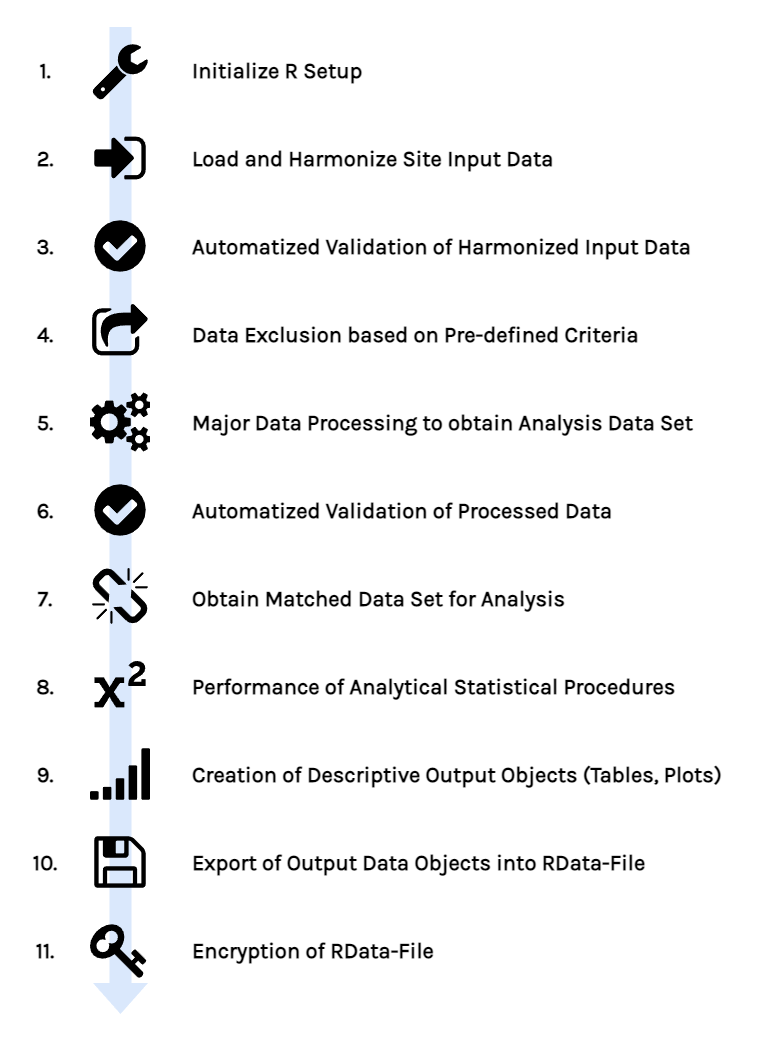
\includegraphics[width=0.7\textwidth,height=\textheight]{Images/AnalysisPipeline.png}

}

\end{figure}

\hypertarget{harmonized-input-data-model}{%
\section{Harmonized Input Data
Model}\label{harmonized-input-data-model}}

\begin{longtable*}{lllll}
\toprule
Attribute Name & Attribute Data Type & Value Format & Value Restrictions & Example Value \\ 
\midrule
\multicolumn{5}{l}{df\_Cases} \\ 
\midrule
PatientPseudonym & character &  &  &  \\ 
CasePseudonym & character &  &  &  \\ 
YearOfBirth & integer & 9999 & [1890 - 2006] & "1975" \\ 
Sex & factor & c & \{w, m, u, d, x\} & "w" \\ 
PostalCode & character & 99999 &  & "35398" \\ 
AdmissionDate & date & YYYY-mm-dd & [2005-01-01 - 2022-12-31] & "2010-07-28" \\ 
AdmissionAge & integer &  & [18 - 120] & "56" \\ 
DischargeDate & date & YYYY-mm-dd & [2005-01-01 - 2022-12-31] & "2014-04-17" \\ 
DischargeReason & factor & 999 & \{01x, 02x, 03x, 04x, 059, 06x, 079, 089, 09x, 10x, 11x, 139, 14x, 15x, 179, 2x9, 309\} & "069" \\ 
\midrule
\multicolumn{5}{l}{df\_CasesICD} \\ 
\midrule
CasePseudonym & character &  &  &  \\ 
DiagnosisType & factor & CC & \{'HD', 'ND'\} & "HD" \\ 
ICDVersion & integer & 9999 & [1990 - 2023] & "2016" \\ 
ICDCode & character & C99.x &  & "C34.1" \\ 
SecondaryICDCode & character & C99.x &  & "Z92.6" \\ 
\midrule
\multicolumn{5}{l}{df\_CasesOPS} \\ 
\midrule
CasePseudonym & character &  &  &  \\ 
OPSVersion & integer & 9999 & [1990 - 2023] & "2007" \\ 
OPSCode & character & 9999xx &  & "12658" \\ 
OPSDate & date & YYYY-mm-dd & [2005-01-01 - 2022-12-31] & "2006-11-25" \\ 
\bottomrule
\end{longtable*}

\hypertarget{processed-data-model}{%
\section{Processed Data Model}\label{processed-data-model}}

\begin{longtable*}{lllllll}
\toprule
Attribute Name & Attribute Data Type & Value Unit & Value Format & Value Restrictions & Example Value & Processing Comment \\ 
\midrule
\multicolumn{7}{l}{df\_DiagnosticCodes} \\ 
\midrule
PatientPseudonym & character &  &  &  &  & Unprocessed from Input Data \\ 
CasePseudonym & character &  &  &  &  & Unprocessed from Input Data \\ 
AdmissionDate & date &  & YYYY-mm-dd & [2005-01-01 - 2022-12-31] & "2010-07-28" & Unprocessed from Input Data \\ 
AdmissionYear & integer &  & YYYY & [2005 - 2022] & "2007" & From AdmissionDate \\ 
AdmissionAge & integer & years &  & [18 - 120] & "56" & Unprocessed from Input Data \\ 
DischargeDate & date &  & YYYY-mm-dd & [2005-01-01 - 2022-12-31] & "2014-04-17" & Unprocessed from Input Data \\ 
DischargeReason & factor &  & 999 & \{01x, 02x, 03x, 04x, 059, 06x, 079, 089, 09x, 10x, 11x, 139, 14x, 15x, 179, 2x9, 309\} & "069" & Unprocessed from Input Data \\ 
DischargeGroup & character &  &  &  & "Rehabilitation or Residential Care" & Meta Data Lookup / Grouping \\ 
LengthOfStay & integer & days &  & > 0 & "134" & DischargeDate - AdmissionDate \\ 
PostalCode & character &  & 99999 &  & "35398" & Unprocessed from Input Data \\ 
DiagnosisType & factor &  & CC & \{'HD', 'ND'\} & "HD" & Unprocessed from Input Data \\ 
ICDCodeShort & character &  & C99 &  & "C34" & String Modification (ICDCode) \\ 
DiagnosisGeneral & character &  &  &  & "Dammriss unter der Geburt" & Meta Data Lookup \\ 
ICDCode & character &  & C99.x &  & "C34.1" & Unprocessed from Input Data \\ 
SecondaryICDCode & character &  & C99.x &  & "Z92.6" & Unprocessed from Input Data \\ 
DiagnosisDetail & character &  &  &  & "Dammriss 1. Grades unter der Geburt" & Meta Data Lookup \\ 
HIVDiseaseGerman & character &  &  &  & "HIV-assoziierte Polyneuropathie" & Meta Data Lookup \\ 
HIVDiseaseClass & factor &  &  & \{'Cancer', 'HIV proprietary', 'Infection'\} & "Infection" & Meta Data Lookup \\ 
HIVInformationClass & factor &  &  & \{'CD4+ count', 'HIV Stadium'\} & "HIV Stadium" & Meta Data Lookup \\ 
HIVInformationValue & character &  &  &  & "B" & Meta Data Lookup \\ 
HIVCodingPlausibility & factor &  &  & \{'Implausible', 'Plausible'\} & "Plausible" & Meta Data Lookup \\ 
HIVStatusInterpretation & factor &  &  & \{'AIDS', 'HIV positive'\} & "AIDS" & Meta Data Lookup \\ 
HIVAssociation & factor &  &  & \{'AIDS defining', 'HIV associated'\} & "HIV associated" & Meta Data Lookup \\ 
IsCancerCode & logical &  &  & \{TRUE, FALSE\} & "FALSE" & Meta Data Lookup / Classification \\ 
IsPotentialMainCancer & logical &  &  & \{TRUE, FALSE\} & "FALSE" &  \\ 
IsPresumedMainCancerDiagnosis & logical &  &  & \{TRUE, FALSE\} & "FALSE" &  \\ 
IsMetastasisCode & logical &  &  & \{TRUE, FALSE\} & "FALSE" & Meta Data Lookup / Classification \\ 
IsPresumedMetastasisDiagnosis & logical &  &  & \{TRUE, FALSE\} & "FALSE" &  \\ 
IsHIVCode & logical &  &  & \{TRUE, FALSE\} & "FALSE" & Meta Data Lookup / Classification \\ 
IsPresumedHIVDiagnosis & logical &  &  & \{TRUE, FALSE\} & "FALSE" &  \\ 
IsAIDSCode & logical &  &  & \{TRUE, FALSE\} & "FALSE" & Meta Data Lookup / Classification \\ 
IsPresumedAIDSDiagnosis & logical &  &  & \{TRUE, FALSE\} & "FALSE" &  \\ 
IsADCode & logical &  &  & \{TRUE, FALSE\} & "FALSE" & Meta Data Lookup / Classification \\ 
IsADCodeCancer & logical &  &  & \{TRUE, FALSE\} & "FALSE" & Meta Data Lookup / Classification \\ 
IsADCodeNonCancerous & logical &  &  & \{TRUE, FALSE\} & "FALSE" & Meta Data Lookup / Classification \\ 
IsHIVNonADCodeCancer & logical &  &  & \{TRUE, FALSE\} & "FALSE" & Meta Data Lookup / Classification \\ 
\midrule
\multicolumn{7}{l}{df\_Patients / df\_PatientsCancer} \\ 
\midrule
PatientPseudonym & character &  &  &  &  & Unprocessed from Input Data \\ 
PatientSubgroup & character &  &  & \{'Cancer+/HIV-', 'Cancer+/HIV+', 'Cancer-/HIV+'\} & "Cancer+/HIV-" &  \\ 
YearOfBirth & integer &  & 9999 & [1890 - 2006] & "1975" &  \\ 
Sex & factor &  & c & \{w, m, u, d, x\} & "w" &  \\ 
PrimaryPostalCode & character &  & 99999 &  & "35398" &  \\ 
PatIsCancerCoded & logical &  &  & \{TRUE, FALSE\} & "FALSE" &  \\ 
PatIsMetastasisCoded & logical &  &  & \{TRUE, FALSE\} & "FALSE" &  \\ 
PatIsHIVCoded & logical &  &  & \{TRUE, FALSE\} & "FALSE" &  \\ 
PatIsAIDSCoded & logical &  &  & \{TRUE, FALSE\} & "FALSE" &  \\ 
CaseCount & integer &  &  & > 0 & "4" &  \\ 
MeanLengthOfStay & double & days &  & > 0 & "7,64" &  \\ 
DistinctCodeCount & integer &  &  & > 0 & "3" &  \\ 
DistinctCodeCountMainCancer & integer &  &  & >= 0 & "2" &  \\ 
DistinctCodeCountHIV & integer &  &  & >= 0 & "2" &  \\ 
DistinctCodeCountAIDS & integer &  &  & >= 0 & "0" &  \\ 
PresumedMainCancerDiagnosisDate & date &  &  &  & "2014-04-17" &  \\ 
PresumedMetastasisDiagnosisDate & date &  &  &  & "2017-10-14" &  \\ 
PresumedHIVDiagnosisDate & date &  &  &  & "2007-08-12" &  \\ 
PresumedAIDSDiagnosisDate & date &  &  &  & "2019-10-02" &  \\ 
FirstMainAdmissionDate & date &  &  & [2005-01-01 - 2022-12-31] & "2006-10-02" &  \\ 
FirstMainAdmissionAge & integer & years &  & [18 - 120] & "56" &  \\ 
LastRecordedDischargeDate & date &  & YYYY-mm-dd & [2005-01-01 - 2022-12-31] & "2014-04-17" &  \\ 
LastRecordedDischargeReason & factor &  & 999 & \{01x, 02x, 03x, 04x, 059, 06x, 079, 089, 09x, 10x, 11x, 139, 14x, 15x, 179, 2x9, 309\} & "069" &  \\ 
FirstMainAdmissionYear & integer &  & 9999 & [2005 - 2022] & "2007" &  \\ 
MainRecordedTimeSpan & integer & days &  &  & "258" &  \\ 
TimeHIVToCancer & integer & days &  &  & "452" &  \\ 
TimeHIVToAIDS & integer & days &  &  & "23" &  \\ 
TimeAIDSToCancer & integer & days &  &  & "0" &  \\ 
TimeCancerToMetastasis & integer & days &  &  & "1254" &  \\ 
ComorbidityScore & integer &  &  &  & "18" & Elixhauser Comorbidity Score \\ 
\midrule
\multicolumn{7}{l}{df\_PatientsCancer} \\ 
\midrule
PatientSubgroupHIVCancerCategory &  &  &  &  &  &  \\ 
PatHadAnyPresumedCancerTherapy &  &  &  &  &  &  \\ 
PatHadSurgery &  &  &  &  &  &  \\ 
PatHadChemotherapy &  &  &  &  &  &  \\ 
PatHadImmunotherapy &  &  &  &  &  &  \\ 
PatHadRadiotherapy &  &  &  &  &  &  \\ 
PatHadNuclearmedTherapy &  &  &  &  &  &  \\ 
PatHadDialysis &  &  &  &  &  &  \\ 
PatHadVentilation &  &  &  &  &  &  \\ 
PatHadComplicationAfterChemo &  &  &  &  &  &  \\ 
TimeChemoToFirstComplication &  &  &  &  &  &  \\ 
TherapyOnset\_1 &  &  &  &  &  &  \\ 
TherapyOnset\_2 &  &  &  &  &  &  \\ 
TherapyOnset\_3 &  &  &  &  &  &  \\ 
TherapyOnset\_4 &  &  &  &  &  &  \\ 
TherapyOnset\_5 &  &  &  &  &  &  \\ 
TherapyOnset\_6 &  &  &  &  &  &  \\ 
OPSDate\_1 &  &  &  &  &  &  \\ 
OPSDate\_2 &  &  &  &  &  &  \\ 
OPSDate\_3 &  &  &  &  &  &  \\ 
OPSDate\_4 &  &  &  &  &  &  \\ 
OPSDate\_5 &  &  &  &  &  &  \\ 
OPSDate\_6 &  &  &  &  &  &  \\ 
\bottomrule
\end{longtable*}

\hypertarget{statistical-methods}{%
\chapter{Statistical Methods}\label{statistical-methods}}

\hfill\break

\hypertarget{descriptive-methods}{%
\section{Descriptive Methods}\label{descriptive-methods}}

\hypertarget{inferential-methods}{%
\section{Inferential Methods}\label{inferential-methods}}

\hypertarget{site-output}{%
\chapter{Site Output}\label{site-output}}

\hfill\break

\hypertarget{output-objects}{%
\section{Output Objects}\label{output-objects}}

\begin{longtable*}{llr}
\toprule
Object Name & Object Attributes & Number of Rows \\ 
\midrule
\multicolumn{3}{l}{Table} \\ 
\midrule
df\_Output\_Age & PatientSubgroup, FirstMainAdmissionYear, AgeGroup, N & 153 \\ 
df\_Output\_Age\_Quantiles & PatientSubgroup, P1, P2.5, P5, P10, P15, P20, P25, P30, P35, P40, P45, P50, P55, P60, P65, P70, P75, P80, P85, P90, P95, P97.5, P99 & 4 \\ 
df\_Output\_Age\_Summary & PatientSubgroup, N, Min, Max, Q1, Median, Q3, MAD, Mean, SD & 4 \\ 
df\_Output\_AgeAtCancerDiagnosis & PatientSubgroup, PresumedMainCancerDiagnosisYear, AgeGroup, N & 109 \\ 
df\_Output\_AgeAtCancerDiagnosis\_Quantiles & PatientSubgroup, P1, P2.5, P5, P10, P15, P20, P25, P30, P35, P40, P45, P50, P55, P60, P65, P70, P75, P80, P85, P90, P95, P97.5, P99 & 3 \\ 
df\_Output\_AgeAtCancerDiagnosis\_Summary & PatientSubgroup, N, Min, Max, Q1, Median, Q3, MAD, Mean, SD & 3 \\ 
df\_Output\_AIDSOccurrence & PatientSubgroup, FirstMainAdmissionYear, N, CountAIDS, ProportionAIDS, CountNoAIDS, ProportionNoAIDS, CountAIDSWithHIVDiagnosis, ProportionAIDSWithHIVDiagnosis, CountAIDSAfterHIVDiagnosis, ProportionAIDSAfterHIVDiagnosis & 30 \\ 
df\_Output\_CancerEntities & PatientSubgroup, PresumedMainCancerCodeFull, N, Proportion & 675 \\ 
df\_Output\_CancerEntities\_OverTime & PatientSubgroup, PresumedMainCancerCodeFull, PresumedMainCancerDiagnosisYear, N, Proportion & 4735 \\ 
df\_Output\_CancerTherapySequence & x, node, next\_x, next\_node & 46025 \\ 
df\_Output\_CancerTopographyDetail & PatientSubgroup, CancerTopographyDetail, N, Proportion & 139 \\ 
df\_Output\_CancerTopographyDetail\_OverTime & PatientSubgroup, CancerTopographyDetail, PresumedMainCancerDiagnosisYear, N, Proportion & 1337 \\ 
df\_Output\_CancerTopographyGroup & PatientSubgroup, CancerTopographyGroup, N, Proportion & 29 \\ 
df\_Output\_CancerTopographyGroup\_OverTime & PatientSubgroup, CancerTopographyGroup, PresumedMainCancerDiagnosisYear, N, Proportion & 371 \\ 
df\_Output\_CaseCount & PatientSubgroup, FirstMainAdmissionYear, CaseCountGroup, N & 173 \\ 
df\_Output\_CaseCount\_Quantiles & PatientSubgroup, P1, P2.5, P5, P10, P15, P20, P25, P30, P35, P40, P45, P50, P55, P60, P65, P70, P75, P80, P85, P90, P95, P97.5, P99 & 4 \\ 
df\_Output\_CaseCount\_Summary & PatientSubgroup, N, Min, Max, Q1, Median, Q3, MAD, Mean, SD & 4 \\ 
df\_Output\_CIS & PatientSubgroup, CancerIsCarcinomaInSitu, PresumedMainCancerDiagnosisYear, N & 58 \\ 
df\_Output\_HIVCancerAIDS & AIDSOccurrence, PresumedMainCancerDiagnosisYear, N & 45 \\ 
df\_Output\_HIVCancerCategories & PatientSubgroup, PatientSubgroupHIVCancerCategory, PresumedMainCancerDiagnosisYear, N & 90 \\ 
df\_Output\_HIVCancerDiagnosisOrder & HIVCancerCategory, HIVCancerDiagnosisOrder, PresumedMainCancerDiagnosisYear, N & 270 \\ 
df\_Output\_HIVCancerEntityCount & PatientSubgroup, N, Min, Max, Q1, Median, Q3, MAD, Mean, SD & 2 \\ 
df\_Output\_HIVCancerSequence & x, node, next\_x, next\_node & 913 \\ 
df\_Output\_LastRecordedDischargeReason & PatientSubgroup, LastRecordedDischargeReason, PresumedMainCancerDiagnosisYear, N, Proportion & 142 \\ 
df\_Output\_MainRecordedTimeSpan\_Quantiles & PatientSubgroup, P1, P2.5, P5, P10, P15, P20, P25, P30, P35, P40, P45, P50, P55, P60, P65, P70, P75, P80, P85, P90, P95, P97.5, P99 & 4 \\ 
df\_Output\_MainRecordedTimeSpan\_Summary & PatientSubgroup, N, Min, Max, Q1, Median, Q3, MAD, Mean, SD & 4 \\ 
df\_Output\_MeanLengthOfStay & PatientSubgroup, FirstMainAdmissionYear, MeanLengthOfStayGroup, N & 180 \\ 
df\_Output\_MeanLengthOfStay\_Quantiles & PatientSubgroup, P1, P2.5, P5, P10, P15, P20, P25, P30, P35, P40, P45, P50, P55, P60, P65, P70, P75, P80, P85, P90, P95, P97.5, P99 & 4 \\ 
df\_Output\_MeanLengthOfStay\_Summary & PatientSubgroup, N, Min, Max, Q1, Median, Q3, MAD, Mean, SD & 4 \\ 
df\_Output\_MetastasisOccurrence & PatientSubgroup, PresumedMainCancerDiagnosisYear, N, CountMetastasis, ProportionMetastasis, CountNoMetastasis, ProportionNoMetastasis, CountMetastasisWithCancerDiagnosis, ProportionMetastasisWithCancerDiagnosis, CountMetastasisAfterCancerDiagnosis, ProportionMetastasisAfterCancerDiagnosis & 30 \\ 
df\_Output\_PostalCodeCounts & PatientSubgroup, PrimaryPostalCode, FirstMainAdmissionYear, Count, Percentage & 3133 \\ 
df\_Output\_SampleSize & PatientSubgroup, FirstMainAdmissionYear, N & 45 \\ 
df\_Output\_Sex & PatientSubgroup, FirstMainAdmissionYear, Sex, N & 92 \\ 
df\_Output\_TherapyComplications & PatientSubgroup, PresumedMainCancerDiagnosisYear, N, CountAnyMajorTherapy, ProportionAnyMajorTherapy, CountChemotherapy, ProportionChemotherapy, CountNoChemotherapy, ProportionNoChemotherapy, CountComplicationAfterChemotherapy, ProportionComplicationAfterChemotherapy, CountNoComplicationAfterChemotherapy, ProportionNoComplicationAfterChemotherapy & 30 \\ 
df\_Output\_TherapyModalities & PatientSubgroup, PresumedMainCancerDiagnosisYear, N, CountNoMajorTherapyCoded, CountAnyMajorTherapy, CountSurgery, ProportionSurgery, CountChemotherapy, ProportionChemotherapy, CountOtherImmunotherapy, ProportionOtherImmunotherapy, CountRadiotherapy, ProportionRadiotherapy, CountNuclearMedicineTherapy, ProportionNuclearMedicineTherapy & 30 \\ 
df\_Output\_TimeCancerToMetastasis\_Quantiles & PatientSubgroup, P1, P2.5, P5, P10, P15, P20, P25, P30, P35, P40, P45, P50, P55, P60, P65, P70, P75, P80, P85, P90, P95, P97.5, P99 & 3 \\ 
df\_Output\_TimeCancerToMetastasis\_Summary & PatientSubgroup, N, Min, Max, Q1, Median, Q3, MAD, Mean, SD & 3 \\ 
\midrule
\multicolumn{3}{l}{eCDF Object} \\ 
\midrule
ls\_Output\_Age\_ECDF & PatientSubgroup, eCDF &  \\ 
ls\_Output\_AgeAtCancerDiagnosis\_ECDF & PatientSubgroup, eCDF &  \\ 
ls\_Output\_CaseCount\_ECDF & PatientSubgroup, eCDF &  \\ 
ls\_Output\_MainRecordedTimeSpan\_ECDF & PatientSubgroup, eCDF &  \\ 
ls\_Output\_MeanLengthOfStay\_ECDF & PatientSubgroup, eCDF &  \\ 
ls\_Output\_TimeCancerToMetastasis\_ECDF & PatientSubgroup, eCDF &  \\ 
ls\_Output\_TimeChemoToComplication\_ECDF & PatientSubgroup, eCDF &  \\ 
\midrule
\multicolumn{3}{l}{Model Object} \\ 
\midrule
model\_Output\_TimeCancerToMetastasis &  &  \\ 
model\_Output\_TimeCancerToMetastasis\_CoxRegression &  &  \\ 
model\_Output\_TimeChemoToComplication &  &  \\ 
model\_Output\_TimeChemoToComplication\_CoxRegression &  &  \\ 
\midrule
\multicolumn{3}{l}{Plot Object} \\ 
\midrule
plot\_Output\_Age &  &  \\ 
plot\_Output\_Age\_OverTime &  &  \\ 
plot\_Output\_AgeAtCancerDiagnosis &  &  \\ 
plot\_Output\_AgeAtCancerDiagnosis\_OverTime &  &  \\ 
plot\_Output\_AnyMajorTherapy &  &  \\ 
plot\_Output\_AnyMajorTherapy\_OverTime &  &  \\ 
plot\_Output\_CancerTopographyDetail &  &  \\ 
plot\_Output\_CancerTopographyGroup &  &  \\ 
plot\_Output\_CaseCount &  &  \\ 
plot\_Output\_CaseCount\_Cancer &  &  \\ 
plot\_Output\_CaseCount\_OverTime &  &  \\ 
plot\_Output\_Chemotherapy\_OverTime &  &  \\ 
plot\_Output\_CIS\_OverTime &  &  \\ 
plot\_Output\_HIVCancerCategories\_OverTime &  &  \\ 
plot\_Output\_LastRecordedDischargeReason &  &  \\ 
plot\_Output\_MainRecordedTimeSpan &  &  \\ 
plot\_Output\_MeanLengthOfStay &  &  \\ 
plot\_Output\_MeanLengthOfStay\_Cancer &  &  \\ 
plot\_Output\_MeanLengthOfStay\_OverTime &  &  \\ 
plot\_Output\_MetastasisOccurrence &  &  \\ 
plot\_Output\_MetastasisOccurrence\_OverTime &  &  \\ 
plot\_Output\_NuclearMedicineTherapy\_OverTime &  &  \\ 
plot\_Output\_OtherImmunotherapy\_OverTime &  &  \\ 
plot\_Output\_Radiotherapy\_OverTime &  &  \\ 
plot\_Output\_SampleSize &  &  \\ 
plot\_Output\_Sex &  &  \\ 
plot\_Output\_Surgery\_OverTime &  &  \\ 
plot\_Output\_TherapyComplications &  &  \\ 
plot\_Output\_TherapyComplications\_OverTime &  &  \\ 
plot\_Output\_TherapyModalities &  &  \\ 
plot\_Output\_TimeCancerToMetastasis &  &  \\ 
plot\_Output\_TimeChemoToComplication &  &  \\ 
\midrule
\multicolumn{3}{l}{Meta Data} \\ 
\midrule
ValidationReport\_df\_Cases & i, type, columns, values, precon, active, eval, units, n\_pass, f\_pass, W, S, N, extract &  \\ 
ValidationReport\_df\_CasesICD & i, type, columns, values, precon, active, eval, units, n\_pass, f\_pass, W, S, N, extract &  \\ 
ValidationReport\_df\_CasesOPS & i, type, columns, values, precon, active, eval, units, n\_pass, f\_pass, W, S, N, extract &  \\ 
ValidationReport\_df\_DiagnosticCodes & i, type, columns, values, precon, active, eval, units, n\_pass, f\_pass, W, S, N, extract &  \\ 
ValidationReport\_df\_PatientsCancer & i, type, columns, values, precon, active, eval, units, n\_pass, f\_pass, W, S, N, extract &  \\ 
\bottomrule
\end{longtable*}

\hypertarget{limitations-and-concerns}{%
\chapter{Limitations and Concerns}\label{limitations-and-concerns}}

\hfill\break
The following chapter provides notes on \textbf{general limitations} and
\textbf{detailed concerns} that occurred during analysis and may present
potential origins of bias. All notes have been assigned to a level of
estimated potential impact (Major, Medium, Minor).

\hypertarget{general-limitations}{%
\section{General Limitations}\label{general-limitations}}

\begin{longtable*}{cc}
\toprule
Limitation & Comment \\ 
\midrule
\bottomrule
\end{longtable*}

\hypertarget{detailed-concerns}{%
\section{Detailed Concerns}\label{detailed-concerns}}

\begin{longtable*}{lc}
\toprule
Concern & Comment \\ 
\midrule
\multicolumn{2}{l}{Major} \\ 
\midrule
Disease onsets may be assumed wrongfully (as too late). Therefore, calculated onset intervals may be incorrect. &  \\ 
If a patient has more than one distinct cancer entity, therapy measures can not be linked to different entities. &  \\ 
\midrule
\multicolumn{2}{l}{Medium} \\ 
\midrule
No causal attribution of complication occurrence to Chemotherapy &  \\ 
\midrule
\multicolumn{2}{l}{Minor} \\ 
\midrule
Age at Admission not exact due to lack of exact birth date. &  \\ 
Occurrence of implausible HIV coding. &  \\ 
Postal code of patient taken from first admission, although moving between admissions is imaginable. &  \\ 
\bottomrule
\end{longtable*}

\part{Publications}

\hypertarget{publications-1}{%
\chapter{Publications}\label{publications-1}}

\hypertarget{publications-2}{%
\section{Publications}\label{publications-2}}

\begin{longtable*}{lllrrlc}
\toprule
Publication Type & Full Title & Event & Submission Date & Publication Date & Authors & Link \\ 
\midrule
\multicolumn{7}{l}{Published} \\ 
\midrule
Abstract & Epidemiology and Inpatient Care Characteristics of HIV-positive Cancer Patients: Exploration of Real World Data from Frankfurt University Hospital & Rhein Main Cancer Retreat 2023 & 1676329200 & 1678834800 & Bastian Reiter, Stefanie Andreas, Daniel Maier, Matthias Müller, Ulrich Seybold, Christoph Stephan, Melanie Stecher, Jörg Janne Vehreschild &  \\ 
Poster & Epidemiology and Inpatient Care Characteristics of HIV-positive Cancer Patients: Exploration of Real World Data from Frankfurt University Hospital & Rhein Main Cancer Retreat 2023 & 1678316400 & 1678921200 & Bastian Reiter, Stefanie Andreas, Daniel Maier, Matthias Müller, Ulrich Seybold, Christoph Stephan, Melanie Stecher, Jörg Janne Vehreschild &  \\ 
\midrule
\multicolumn{7}{l}{Submitted} \\ 
\midrule
Abstract & Epidemiology and Inpatient Care Characteristics of HIV-positive Cancer Patients: Federated Exploration of Real World Data from Four German University Hospitals & 3rd German Cancer Research Congress & 1688940000 &  & Bastian Reiter, Stefanie Andreas, Daniel Maier, Matthias Müller, Ulrich Seybold, Christoph Stephan, Melanie Stecher, Jörg Janne Vehreschild &  \\ 
\midrule
\multicolumn{7}{l}{To be submitted} \\ 
Poster &  & 3rd German Cancer Research Congress &  &  &  &  \\ 
\bottomrule
\end{longtable*}

\part{References}

\hypertarget{references-1}{%
\chapter{References}\label{references-1}}

\hfill\break

\hypertarget{refs}{}
\begin{CSLReferences}{0}{0}
\leavevmode\vadjust pre{\hypertarget{ref-hoffmann2019}{}}%
\CSLLeftMargin{1. }%
\CSLRightInline{Hoffmann, W. \emph{et al.}
\href{https://doi.org/10.1007/s10654-019-00500-x}{Guidelines and
recommendations for ensuring Good Epidemiological Practice (GEP): a
guideline developed by the German Society for Epidemiology}.
\emph{European Journal of Epidemiology} \textbf{34}, 301--317 (2019).}

\leavevmode\vadjust pre{\hypertarget{ref-swart2015}{}}%
\CSLLeftMargin{2. }%
\CSLRightInline{Swart, E. \emph{et al.}
\href{https://doi.org/10.1055/s-0034-1396815}{Gute Praxis
Sekundärdatenanalyse (GPS): Leitlinien und Empfehlungen}. \emph{Das
Gesundheitswesen} \textbf{77}, 120--126 (2015).}

\leavevmode\vadjust pre{\hypertarget{ref-sandve2013}{}}%
\CSLLeftMargin{3. }%
\CSLRightInline{Sandve, G. K., Nekrutenko, A., Taylor, J. \& Hovig, E.
\href{https://doi.org/10.1371/journal.pcbi.1003285}{Ten Simple Rules for
Reproducible Computational Research}. \emph{PLoS Computational Biology}
\textbf{9}, e1003285 (2013).}

\end{CSLReferences}



\end{document}
